\subsection{Integración del sistema}

Una vez elaborado y probado cada uno de los subsistemas, se fueron integrando respetando la relación existente entre cada uno de los módulos elaborados.

La primera parte fue la integración entre los elementos del sistema de procesamiento de la materia, instalando el eje de aireación dentro del contenedor que a su vez, es instalado sobre la estructura principal. Se realizaron pruebas para verificar que el sistema fuera capaz de operar sin algún problema. (Figura \ref{fg:palas_dentro})

 \begin{figure}[h!]
            \centering
            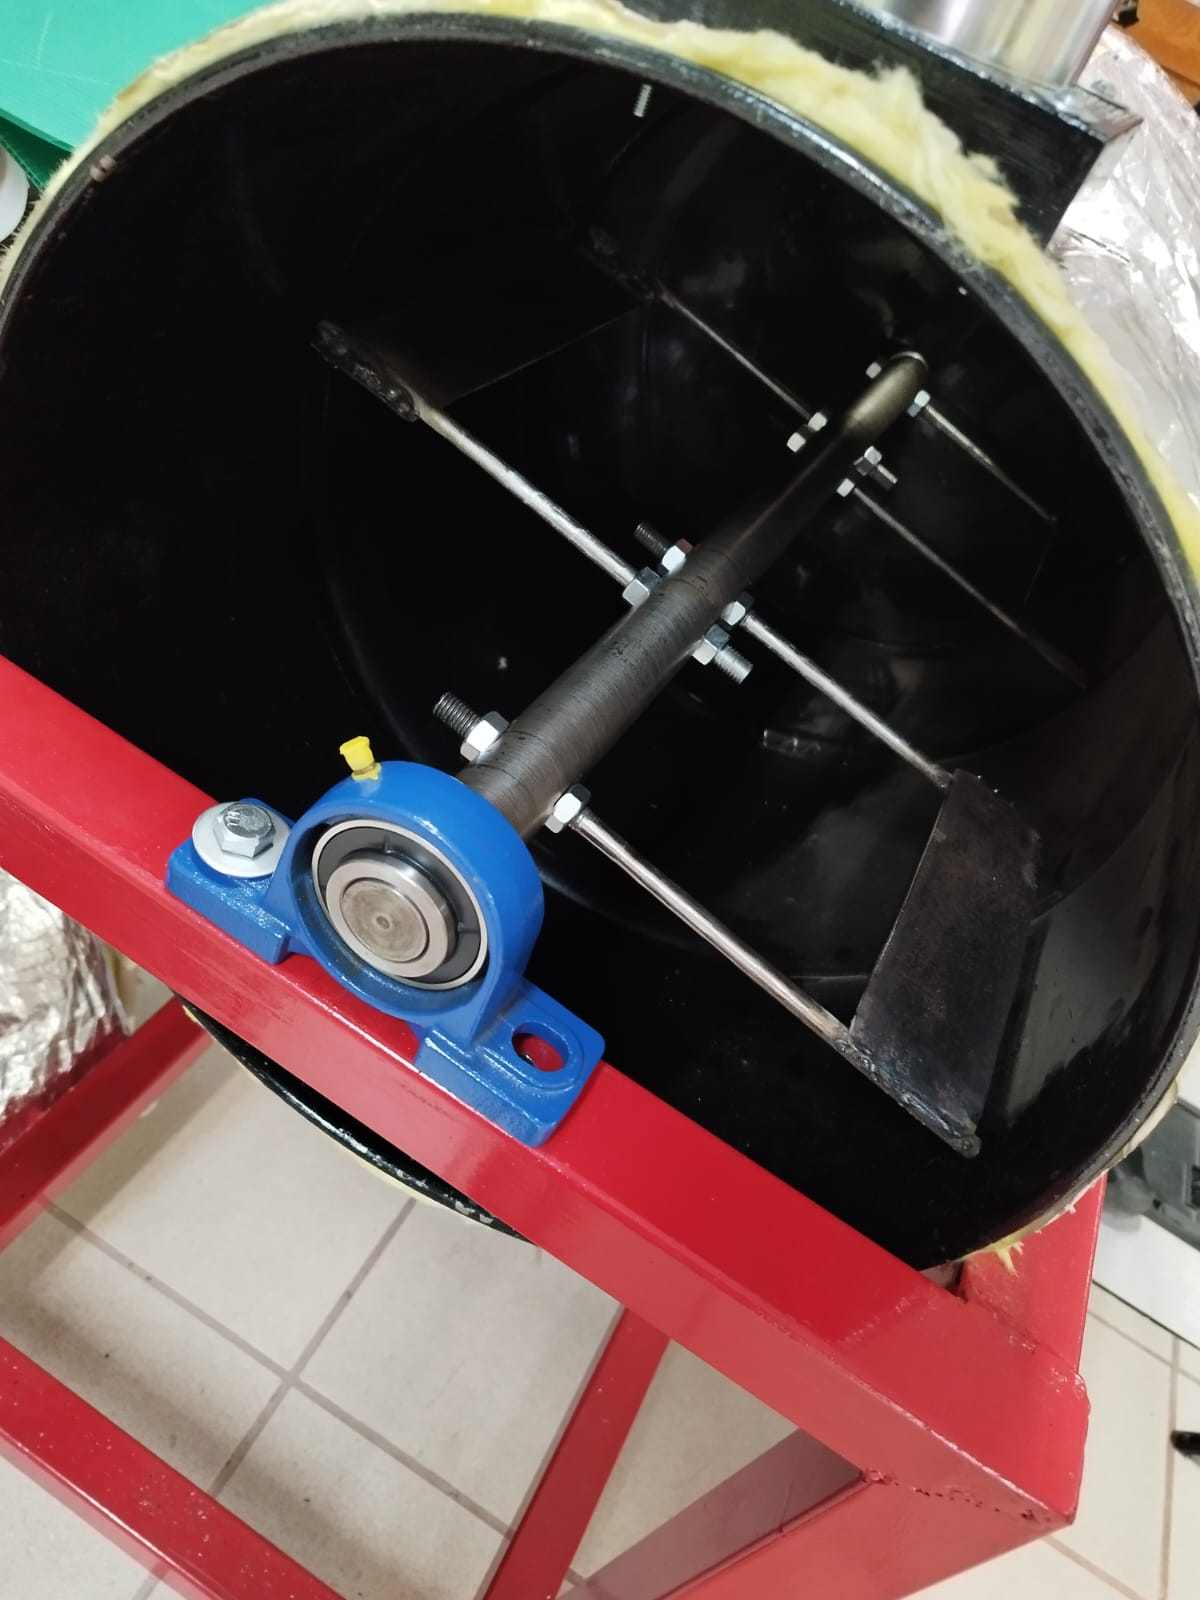
\includegraphics[scale=0.2]{images/Capitulo_Imple/S7/palas_dentro.jpeg}
            \caption{Instalación del eje de aireación dentro del contenedor}
            \label{fg:palas_dentro}
 \end{figure}
 
 \clearpage
Ya con el contenedor instalado dentro la estructura, se realizaron las conexiones entre los elementos de ventilación y trituración, para lo cual, se realizaron perforaciones sobre el contenedor, donde se instalaron y atornillaron las piezas necesarias para sostener los elementos de cada subsistema.

En una de las partes, se coloco la base que sostiene el filtro de olores, la cual está atornillada en la parte final del contenedor, mientras que a la entrada, se coloca la base donde se conectan los conductos de PVC, provenientes del sistema de trituración. (Figura \ref{fg:Filtro_olores}) 

 \begin{figure}[h!]
            \centering
            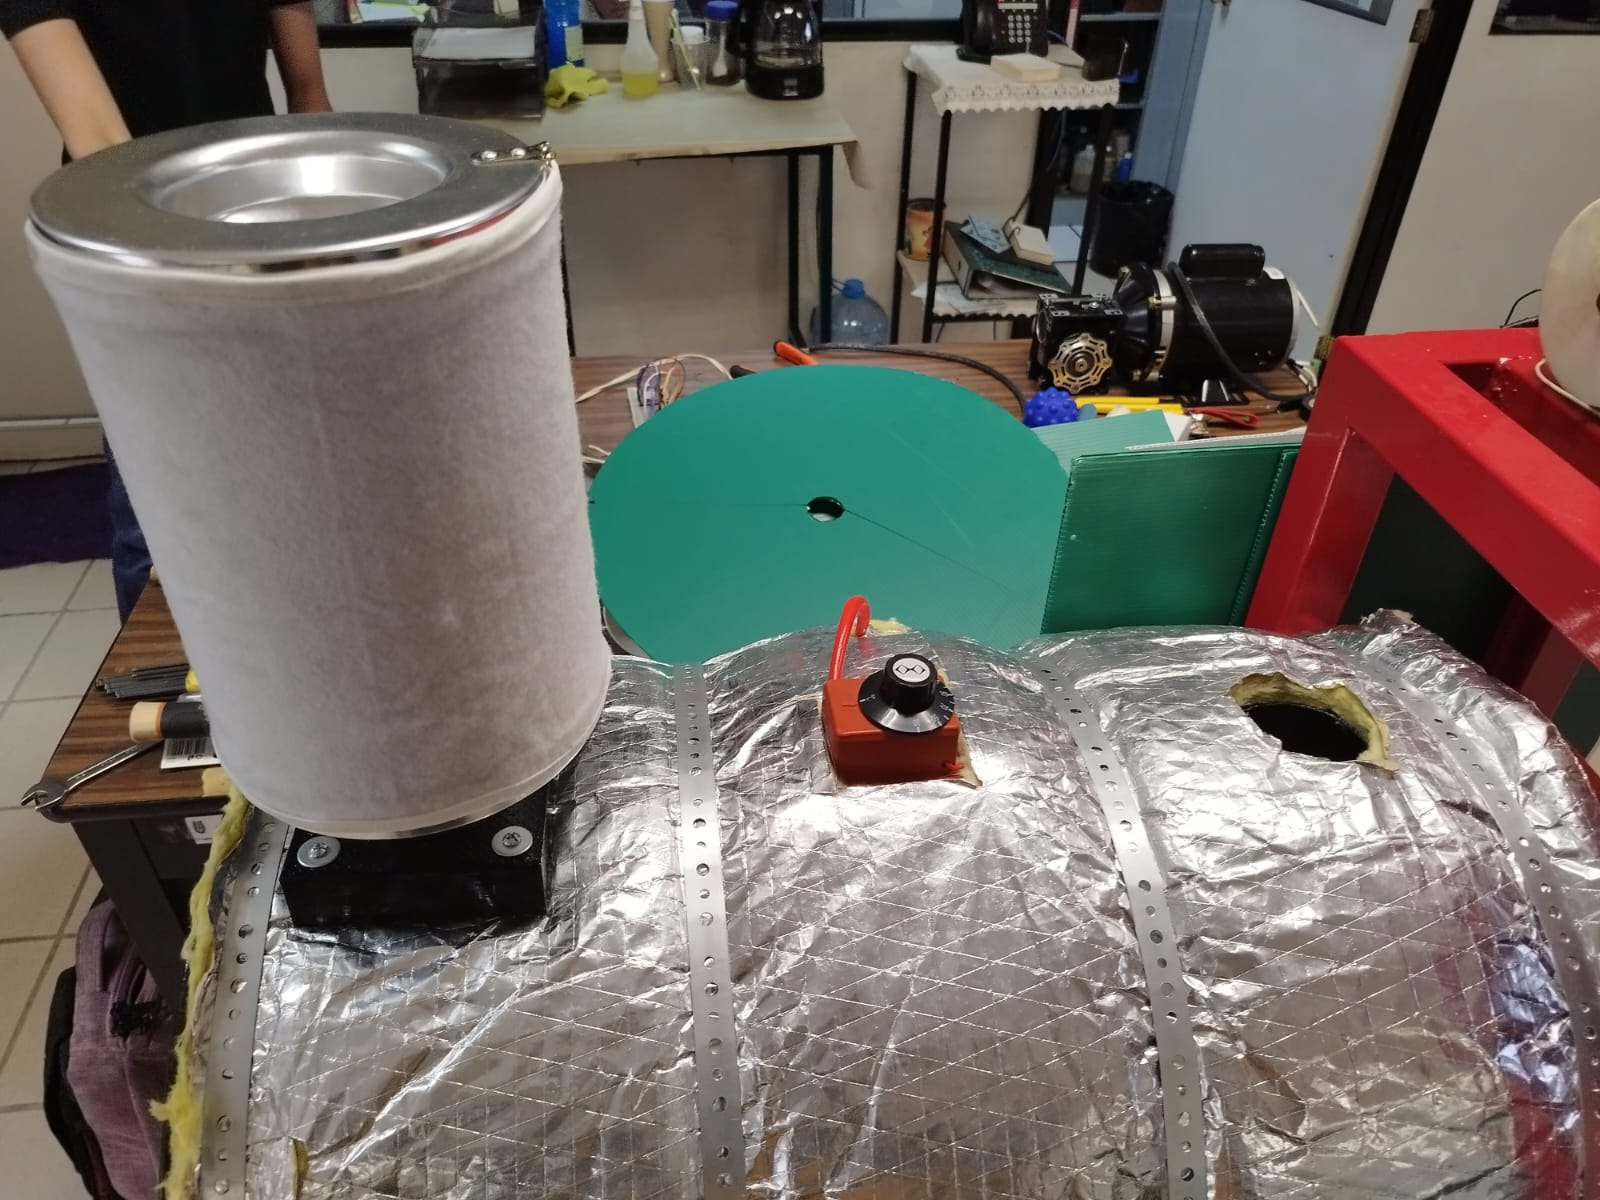
\includegraphics[scale=0.2]{images/Capitulo_Imple/S7/perfora.jpeg}
            \caption{Instalación del filtro de olores}
            \label{fg:Filtro_olores}
 \end{figure}
 
 \clearpage
 También se terminó por instalar el sistema de trituración sobre la estructura, atornillando el molino y su motor. Se ajustó la banda que transmite el movimiento entre el juego poleas y se colocaron los conductos de alimentación al contenedor. (Figura \ref{fg:Instalacion_triturac})

  \begin{figure}[h!]
            \centering
            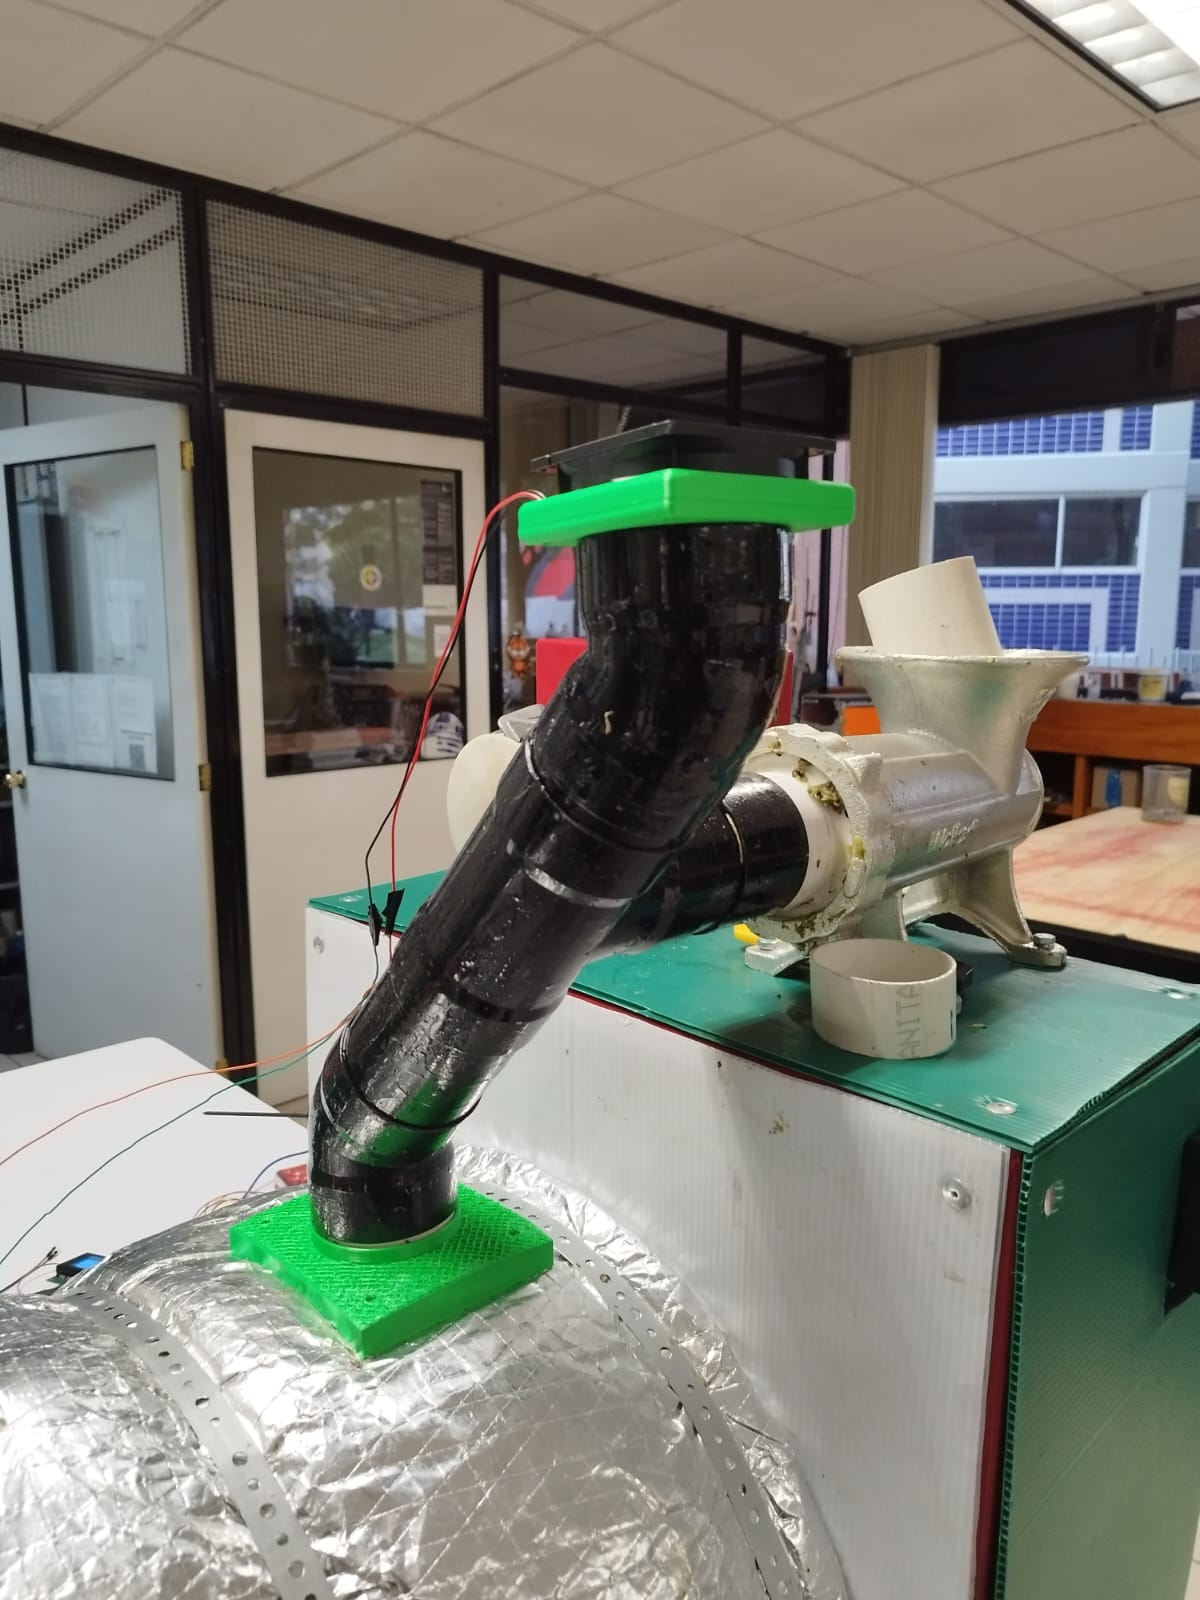
\includegraphics[scale=0.2]{images/Capitulo_Imple/S7/Sal_trituracion.jpeg}
            \caption{Sistema de trituración instalado}
            \label{fg:Instalacion_triturac}
 \end{figure}

\clearpage
Lo siguiente, fue colocar los sensores, recordando que el sensor de humedad se coloca en la parte superior del contenedor, sobre la perforación en la que se encuentra el filtro de olores y el de temperatura en la parte lateral, pegado a la pared del tanque.

Ya con la parte del eje y del contenedor colocada, se realizo del ensamble de los elementos de transmisión de movimiento del eje de aireación, el cual consta del motor eléctrico, el motor-reductor y el juego de poleas, con su respectiva banda. (Figura \ref{fg:Sist_trans_ints})

 \begin{figure}[h!]
            \centering
            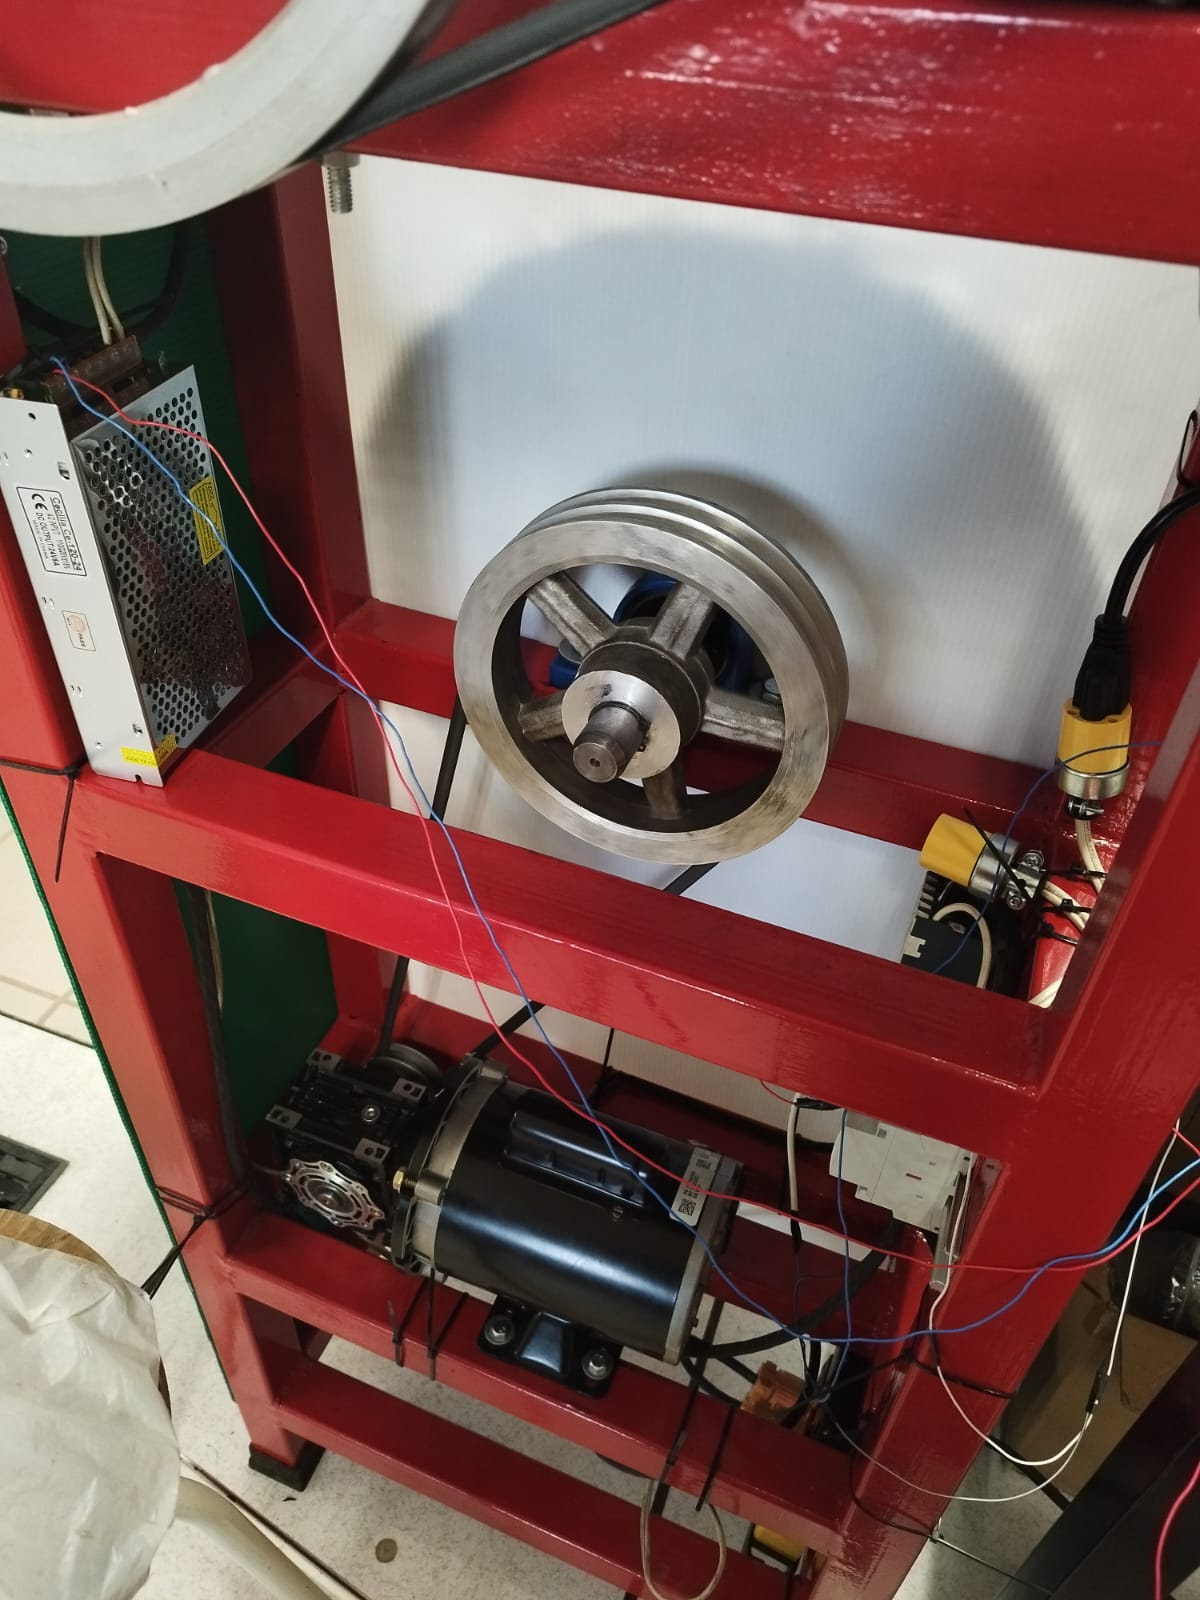
\includegraphics[scale=0.2]{images/Capitulo_Imple/S7/motor.jpeg}
            \caption{Sistema de transmisión instalado}
            \label{fg:Sist_trans_ints}
 \end{figure}

\clearpage
Al final, se colocaron todos los sistemas de control del dispositivo, colocando los contactores en el riel para la activación de los diferentes actuadores eléctricos, así como el montaje de la interfaz a un costado de la estructura. (Figura \ref{fg:Instal_contac})

 \begin{figure}[h!]
            \centering
            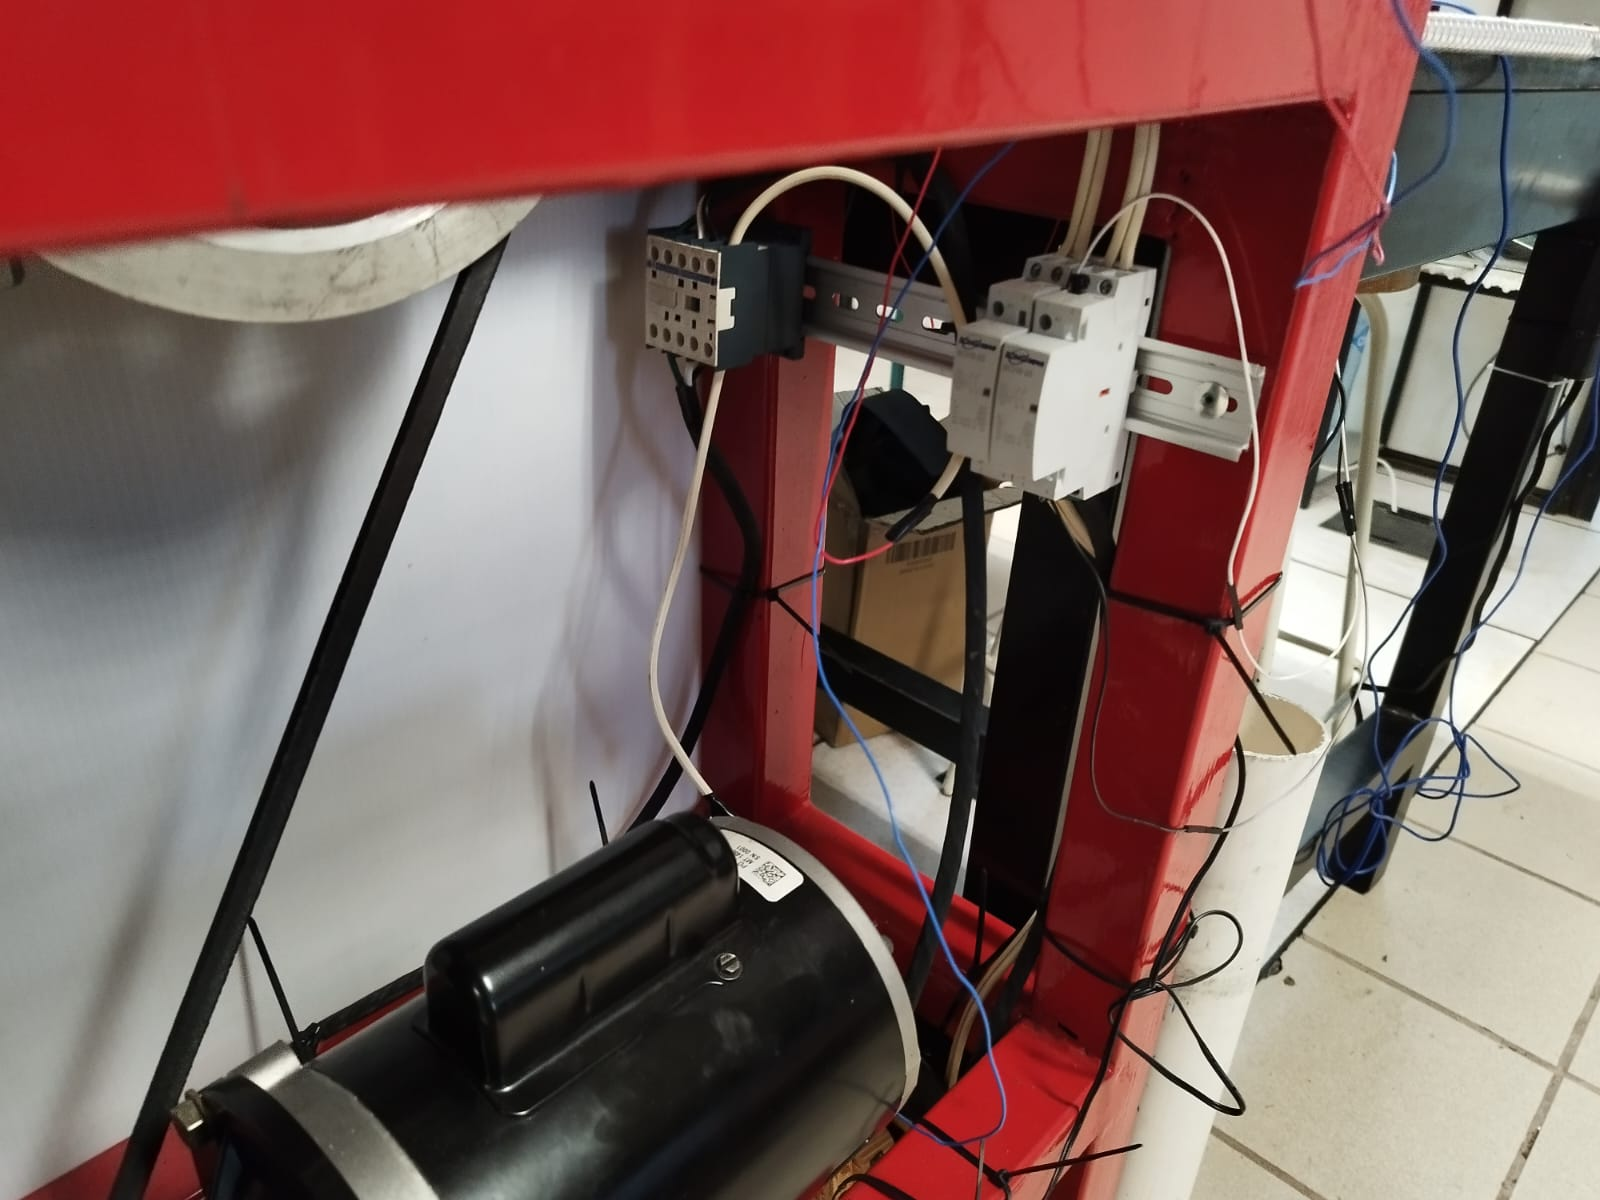
\includegraphics[scale=0.2]{images/Capitulo_Imple/S7/cableado.jpeg}
            \caption{Contantores instalados}
            \label{fg:Instal_contac}
 \end{figure}

De igual forma se colocaron laminas de plástico, encargadas de aislar los elementos mecánicos, eléctricos y electrónicos del sistema, para evitar que estén en contacto directo con el usuario o con líquidos que se puedan presentar durante las etapas del proceso.

\clearpage
Ya con el sistema armado, se realizaron las pruebas necesarias para observar su funcionamiento y realizar los ajustes necesarios para su integración y funcionamiento completo (Figura \ref{fg:sistema integrado})

 \begin{figure}[h!]
            \centering
            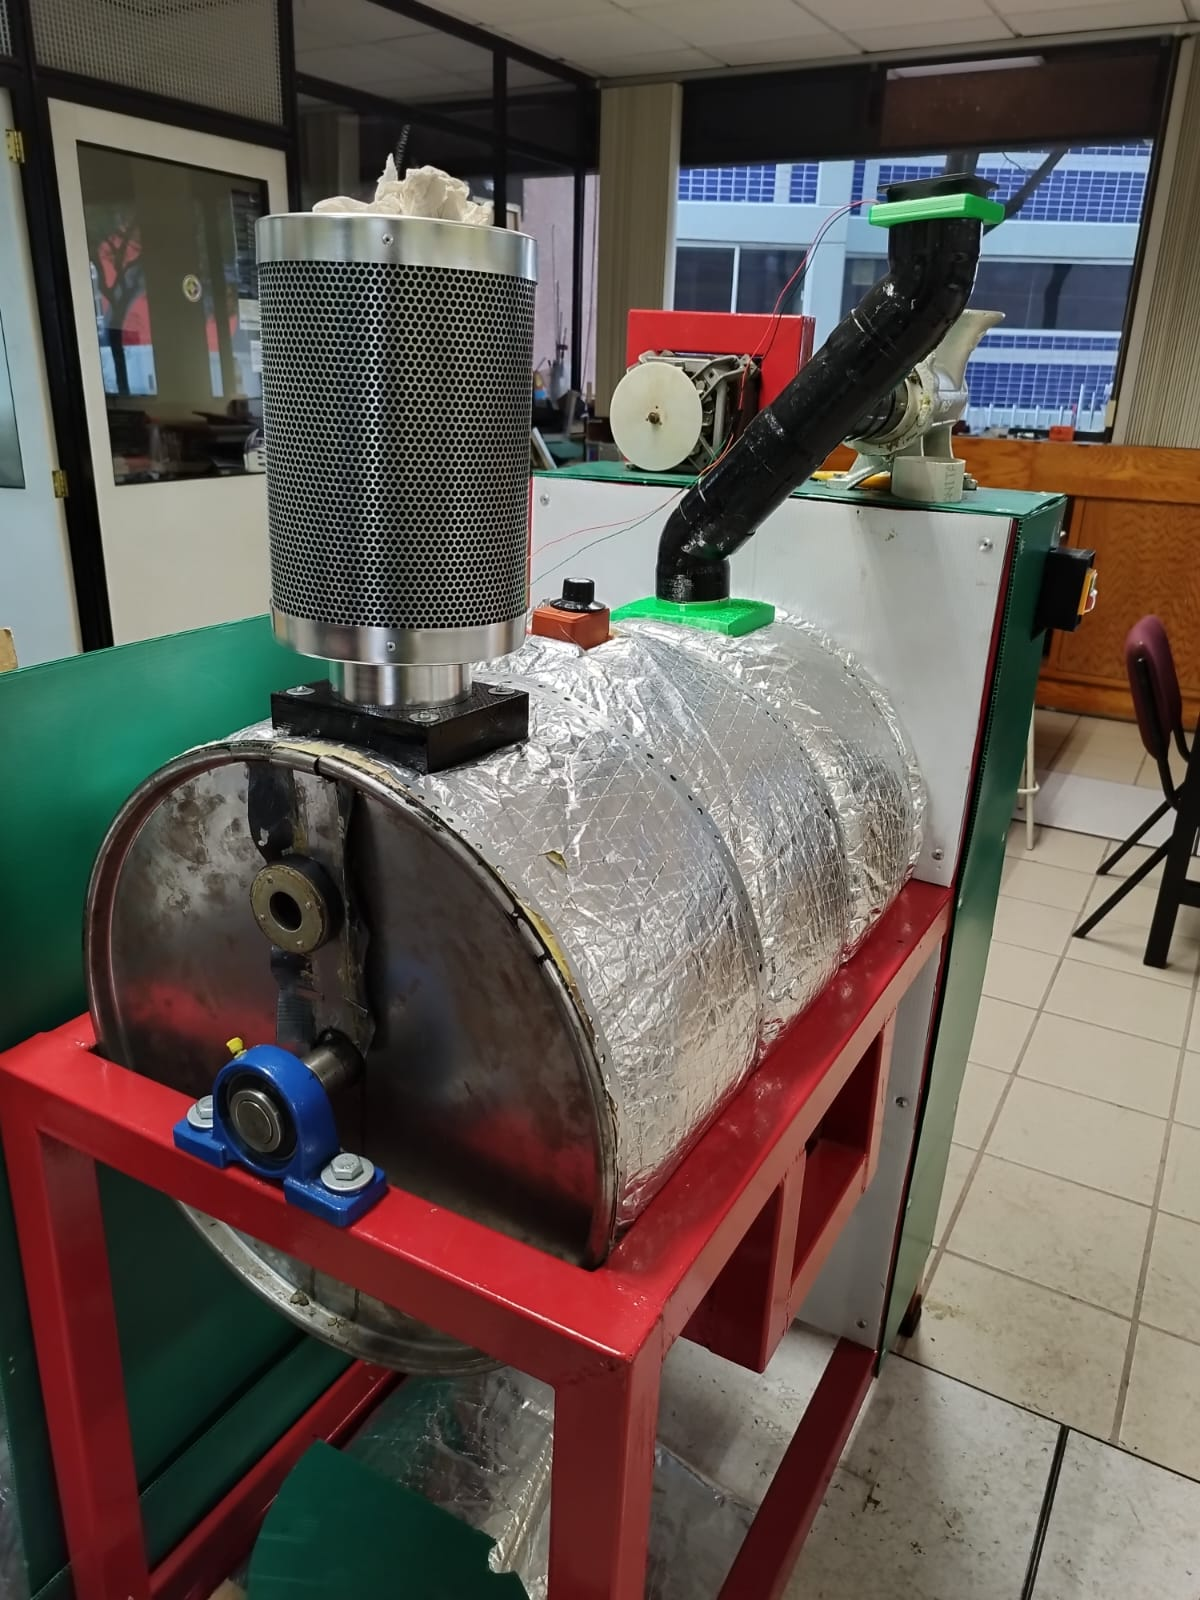
\includegraphics[scale=0.2]{images/Capitulo_Imple/S7/sistema_integrado.jpeg}
            \caption{Muestra del sistema de compostaje completo}
            \label{fg:sistema integrado}
 \end{figure}

 \clearpage